\chapter{TP3 : Outil de simulation de réseaux : NS-2}
  Afin de mieux expliquer le fonctionnement du code proposé, on a commenté le plus de lignes possibles afin de clarifier directement les lignes qui sont découvertes à ce moment. Ainsi, le gros de ce TP se passe principalement dans le code en annexe. Les couleurs ont été rajoutés au sein de la procédure attach-expo-traffic.

  La procédure attach-expo-traffic permet comme son nom l'indique d'attacher aux noeuds 0, 1 et 2 les sources de trafic exponentielles. Celle-ci crée un agent UDP auxquels elle attache simultanément l'agent source de trafic, mais aussi un agent permettant de recevoir ce trafic (LossMonitor). Elle est appelée pour les trois noeuds qui génèreront du trafic, afin de ne pas répéter le code.

  La procédure record convertit ce que les "sink" recoivent en octets afin de les écrire dans les fichiers f0, f1 et f2, puis se rappelle après un certain temps afin de continuer l'enregistrement, en remettant les variables contenant les octets à 0.

  En changeant le temps d'enregistrement des courbes nous obtenons un taux d'échantillonage plus ou moins élevé. Cela nous permet de voir qu'en ayant un taux d'échantillonage trop bas, on a un résultat qui n'est pas exactement la réalité. Le débit ne réduit pas, il s'arrête à certains moments. Ainsi un taux d'échantillonnage de 0,1s, c'est-à-dire le délai impliqué par les connexions, on peut voir les trafics démarrer et s'arrêter, plutôt que réduire et se modifier. On a donc un résultat plus proche de la réalité.
  \clearpage
  \begin{figure}
    \centering
      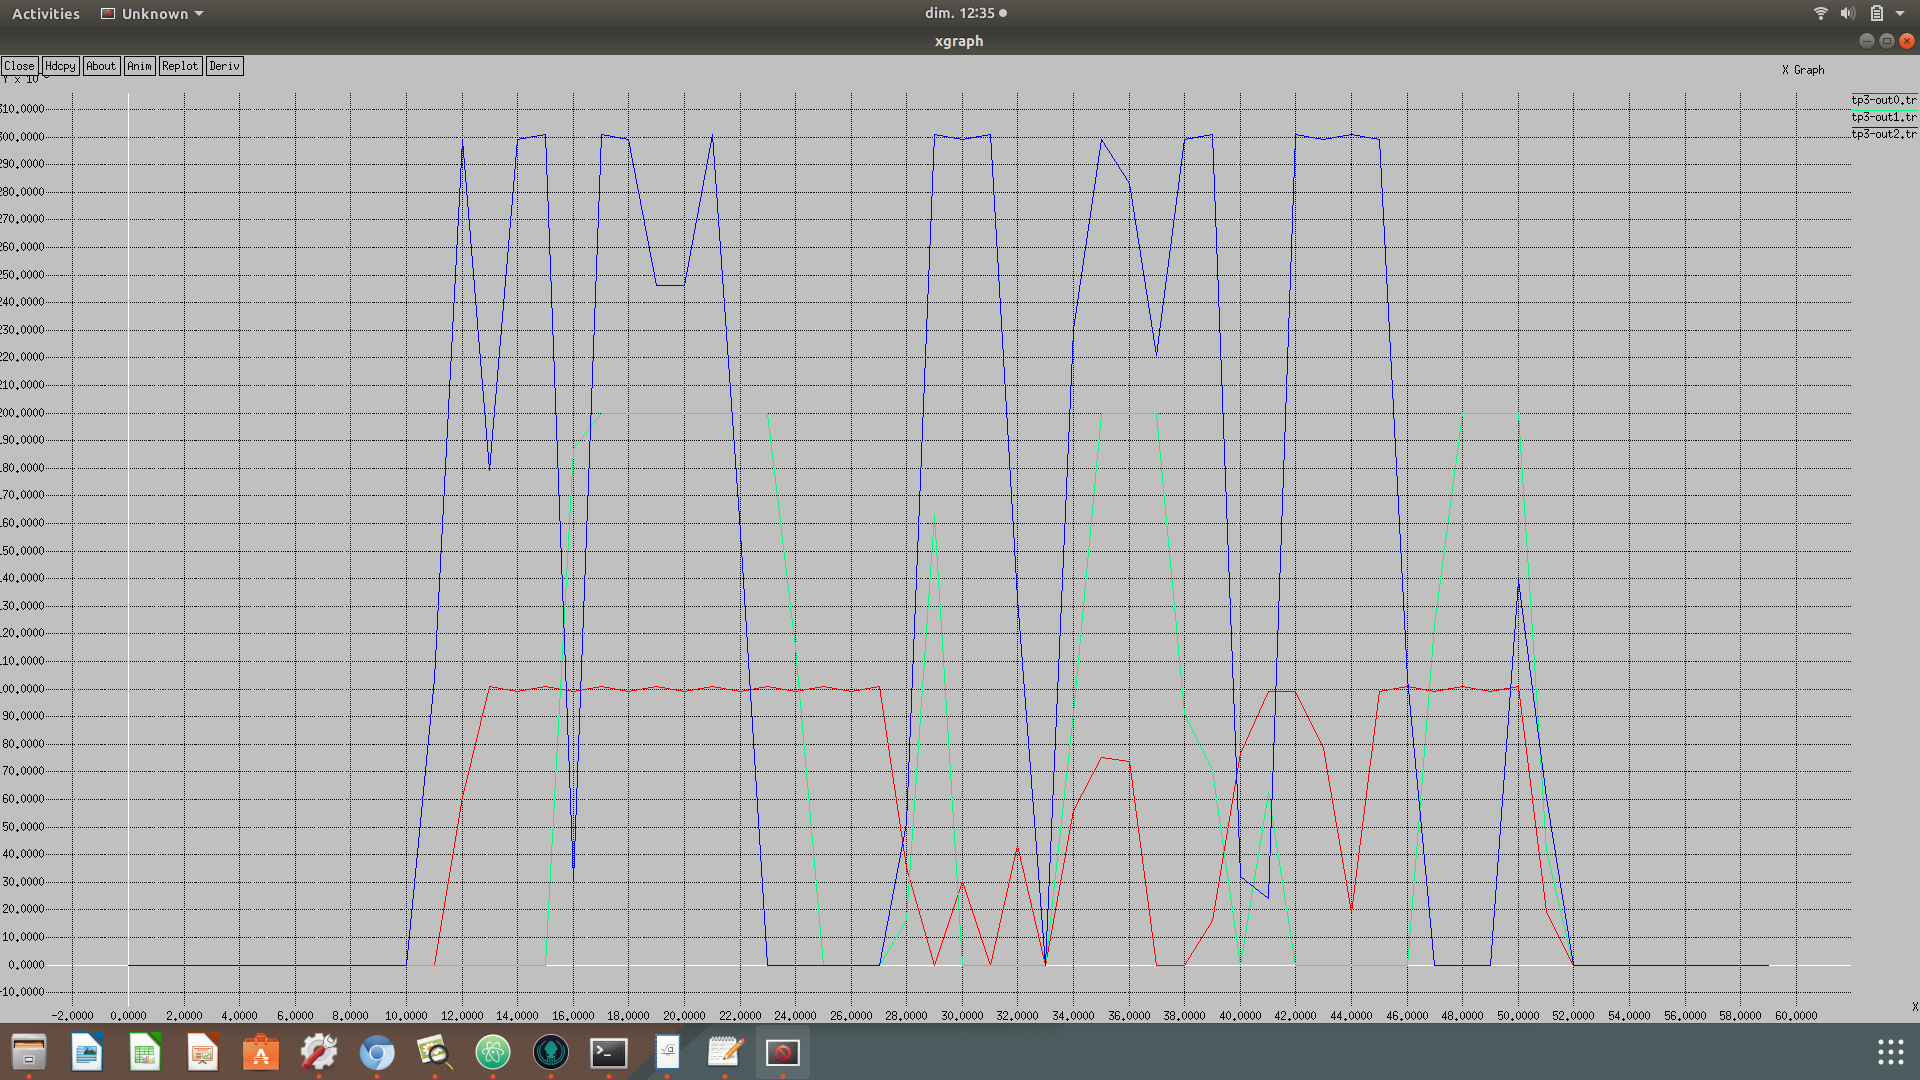
\includegraphics[width=0.99\columnwidth]{./tp3/1,0.png}
      \caption{xGraph : Échantillonage de 1 seconde}
  \end{figure}

  \begin{figure}
    \centering
      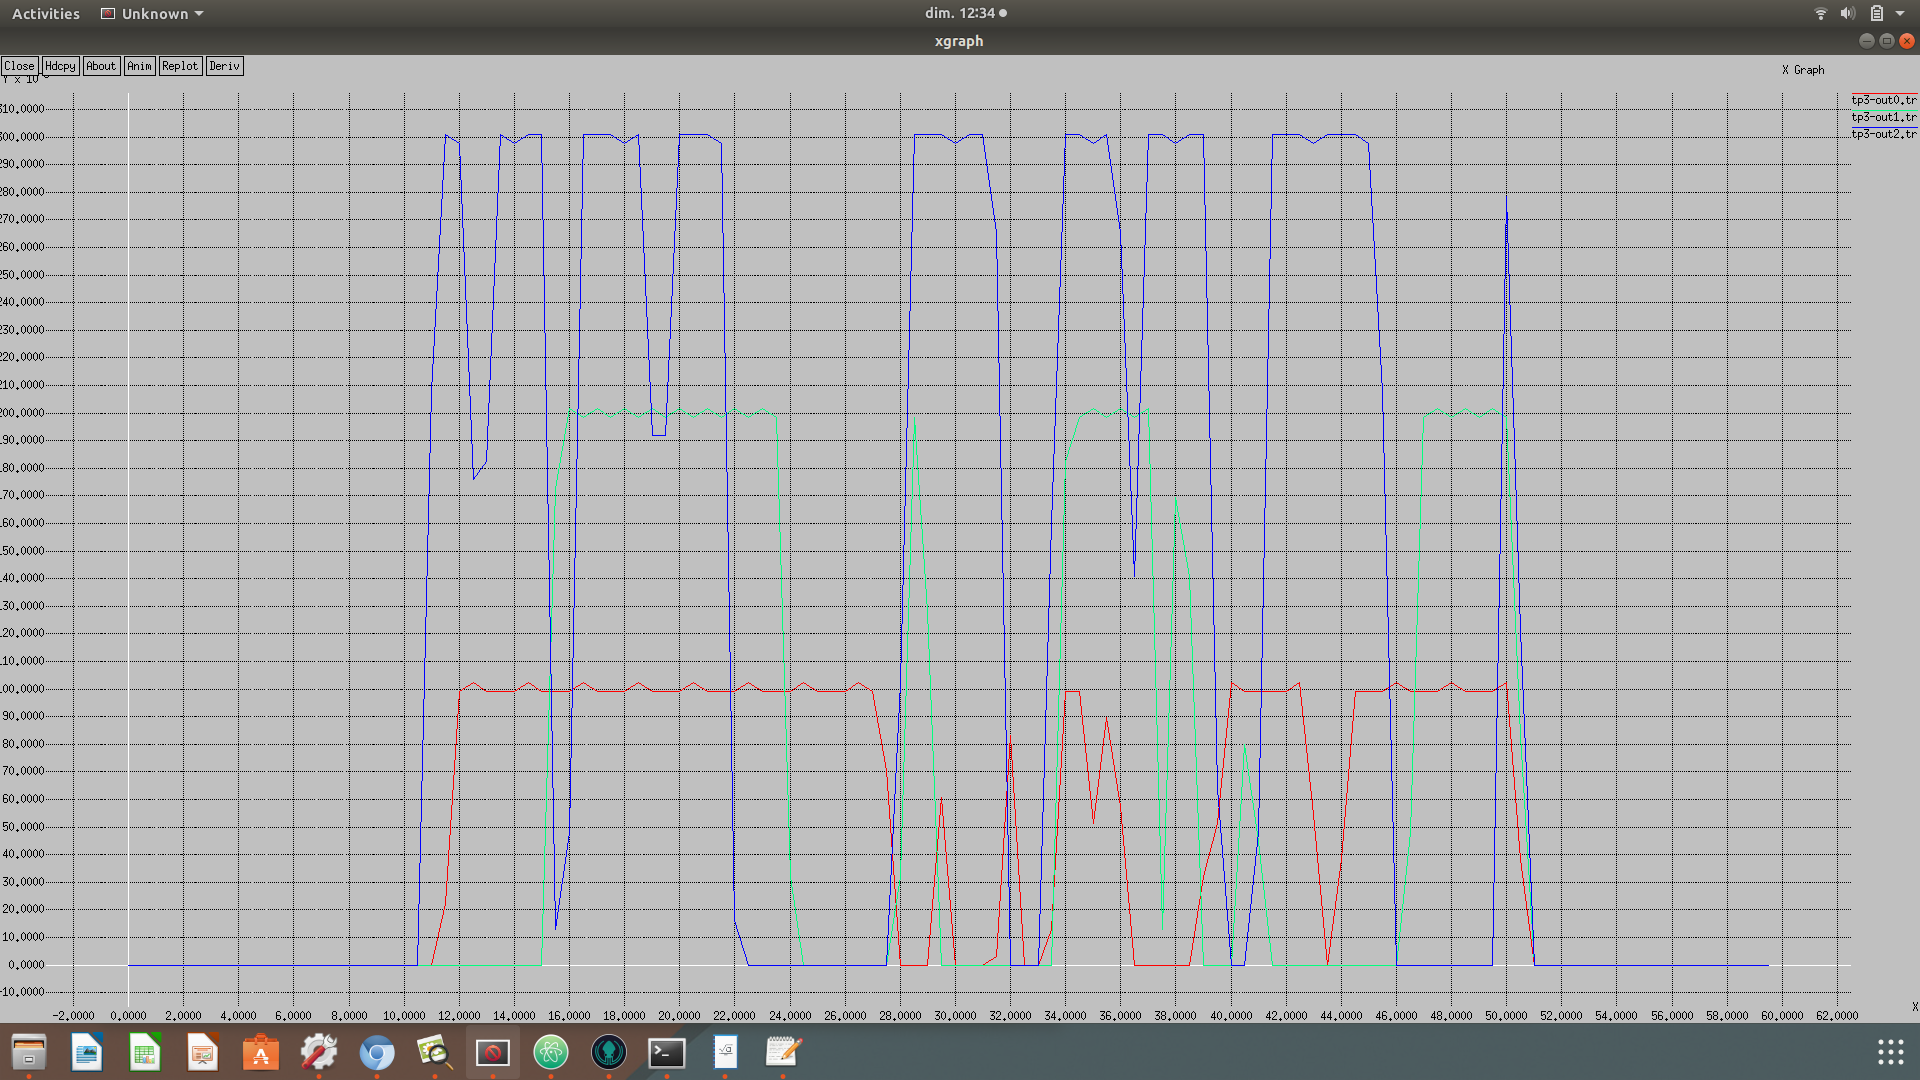
\includegraphics[width=0.99\columnwidth]{./tp3/0,5.png}
      \caption{xGraph : Échantillonage de 0.5 seconde}
  \end{figure}

  \begin{figure}
    \centering
      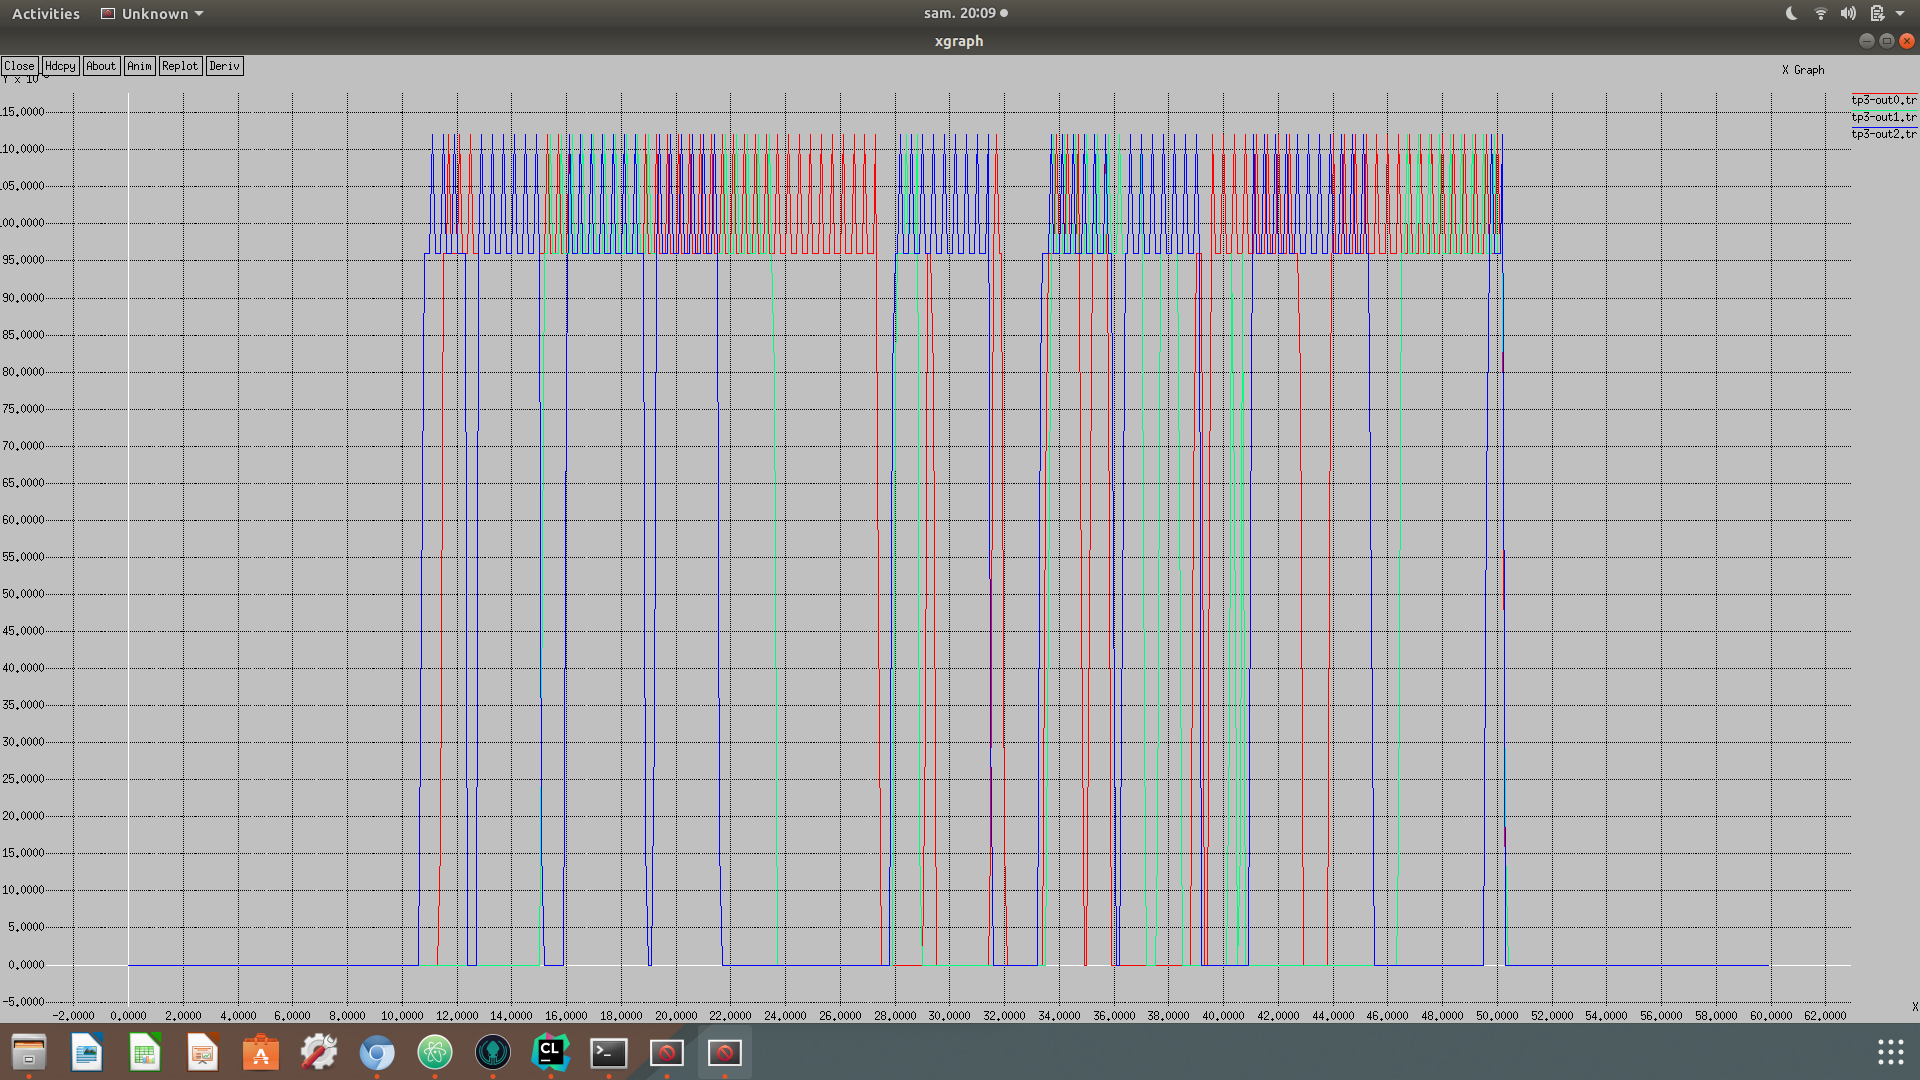
\includegraphics[width=0.99\columnwidth]{./tp3/0,1.png}
      \caption{xGraph : Échantillonage 0.1 seconde}
  \end{figure}
